\chapter{Evaluation und Validierung}\label{ch:evaluation}

In diesem Kapitel wird das entwickelte Gesamtsystem anhand der in Kapitel 5 definierten Anforderungen und Abnahmekriterien bewertet. Ziel ist es, sowohl die Erkennungsleistung der KI-Verarbeitungskette als auch die technische Leistungsfähigkeit des eingebetteten Systems zu untersuchen. Dazu werden die Erkennungsgenauigkeit, das Verhalten unter unterschiedlichen Umgebungsbedingungen, die Verarbeitungsgeschwindigkeit sowie der Speicher- und Ressourcenverbrauch betrachtet.

Die Evaluation umfasst sowohl das Klassifikationsmodell als auch den integrierten Prototyp. Die Bewertung des Modells erfolgt anhand zuvor nicht für das Training verwendeter Testdaten. Ergänzend wird das Gesamtsystem unter festgelegten realen Einsatzbedingungen untersucht. Dadurch kann zwischen der isolierten Modellleistung und der Erkennungsleistung der vollständig integrierten Kamera- und KI-Verarbeitungskette unterschieden werden. Die ermittelten Ergebnisse werden abschließend den festgelegten Anforderungen und Abnahmekriterien gegenübergestellt. Auf dieser Grundlage wird beurteilt, welche Anforderungen vollständig, teilweise oder nicht erfüllt wurden.

\section{Trainingsevaluation}\label{sec:trainingsprozess}

Das Training des Gebärdensprachenmodells wurde über den Verlauf von \textit{Accuracy} und des \textit{Loss} für Trainings- und Validierungsdaten über insgesamt 20 Epochen bewertet. Im folgenden die finalen Trainingsergebnisse:


\subsection{Entwicklung der Accuracy}

\begin{figure}[!h]
    \centering
    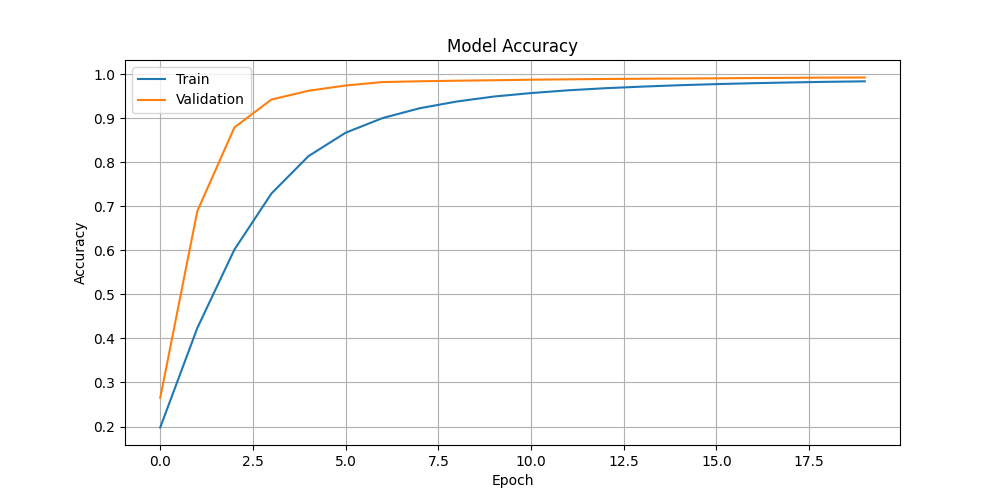
\includegraphics[width=0.9\linewidth]{material/Figure_1.png}
    \caption{Gebärdensprachen-Model Accuracy | Training}
    \label{fig:train-accuracy}
\end{figure}

Zu Beginn des Trainings (Epoche 0) liegt die Trainings-Accuracy bei etwa 20\,\%, während die Validierungs-Accuracy bereits rund 27\,\% beträgt. In den ersten Epochen steigt die Accuracy beider Datensätze deutlich an. Besonders die Validierungs-Accuracy verbessert sich sehr schnell und erreicht bereits nach etwa drei bis fünf Epochen Werte von über 95\,\%.

Die Trainings-Accuracy steigt etwas langsamer, jedoch kontinuierlich, und erreicht gegen Ende des Trainings einen Wert von nahezu 99\,\%. Ab etwa der 10. Epoche flachen beide Kurven deutlich ab, was darauf hindeutet, dass das Modell konvergiert und weitere Epochen nur noch geringe Leistungsverbesserungen bewirken.

Auffällig ist, dass die Validierungs-Accuracy während des gesamten Trainings geringfügig über der Trainings-Accuracy liegt. Dieses Verhalten kann beispielsweise durch Regularisierungsmethoden wie \textit{Dropout} oder \textit{Data Augmentation} erklärt werden und stellt kein Anzeichen für Overfitting dar.

\subsection{Entwicklung der Loss}

\begin{figure}[!h]
    \centering
    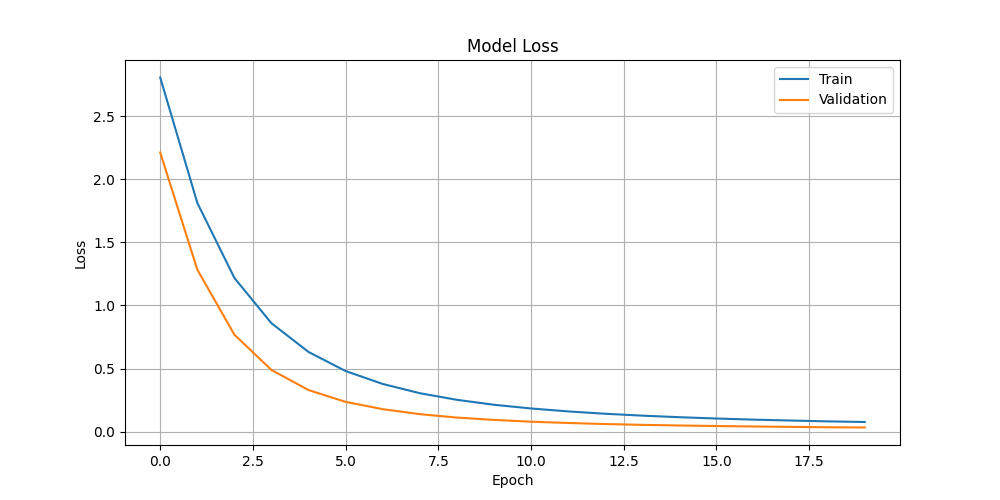
\includegraphics[width=0.9\linewidth]{material/Figure_2.png}
    \caption{Gebärdensprachen-Model Loss | Training}
    \label{fig:train-loss}
\end{figure}

Der Trainings-Loss beginnt bei einem hohen Wert von etwa 2{,}8 und sinkt während der ersten Epochen sehr stark. Anschließend nimmt sie langsamer ab und erreicht am Ende des Trainings einen Wert von ungefähr 0{,}06.

Auch der Validierungs-Loss zeigt einen kontinuierlichen Rückgang von etwa 2{,}2 auf rund 0{,}03. Beide Kurven verlaufen gleichmäßig und nähern sich gegen Ende einem stabilen Minimalwert an.

Besonders hervorzuheben ist, dass der Validierungs-Loss während des gesamten Trainings kontinuierlich sinkt und kein erneuter Anstieg zu beobachten ist. Ein solcher Anstieg würde typischerweise auf Overfitting hindeuten. Da dies hier nicht der Fall ist, kann davon ausgegangen werden, dass das Modell die zugrunde liegenden Muster erfolgreich gelernt hat und diese auf unbekannte Daten gut überträgt.

\subsection{Interpretation}

Aus den dargestellten Trainingskurven lassen sich folgende Erkenntnisse ableiten:

\begin{itemize}
    \item Das Modell lernt bereits in den ersten Epochen sehr effektiv.
    \item Die Accuracy steigt kontinuierlich auf nahezu 99\,\%, während der Loss gleichzeitig gegen Null sinkt.
    \item Trainings- und Validierungskurven verlaufen nahezu parallel.
    \item Es sind keine Anzeichen für Overfitting erkennbar, da die Validierungs-Loss nicht ansteigt und die Validierungs-Accuracy nicht abfällt.
\end{itemize}

\section{Erkennungsgenauigkeit}\label{sec:erkennungsgenauigkeit}

Die Erkennungsgenauigkeit wird zunächst anhand des bei der Modellentwicklung zurückgehaltenen Testdatensatzes und anschließend anhand der praktischen Evaluation des integrierten Gesamtsystems untersucht.
Die erste Auswertung betrachtet ausschließlich die Klassifikationsleistung des Modells auf bereits 
ermittelten Landmark-Daten. Die praktische Evaluation berücksichtigt dagegen die vollständige Verarbeitungskette von der Bildaufnahme über die Handdetektion und Landmark-Erkennung bis zur Zeichenklassifikation.

Zur klassenbezogenen Auswertung werden für beide Versuchsreihen Konfusionsmatrizen erstellt. In einer Konfusionsmatrix werden die tatsächlichen Zeichenklassen den vorhergesagten Klassen gegenübergestellt. Die Einträge auf der Hauptdiagonalen entsprechen korrekten Klassifikationen, während Einträge außerhalb der Hauptdiagonalen Verwechslungen zwischen den Klassen darstellen. \cite{fritzHandGestureRecognition}

Da der Testdatensatz und die praktische Evaluation eine unterschiedliche Anzahl an Beispielen enthalten können, werden für die Gegenüberstellung insbesondere die zeilenweise normalisierten Konfusionsmatrizen verwendet. Dadurch wird für jede tatsächliche Klasse der relative Anteil der jeweiligen Vorhersagen betrachtet. Auf dieser Grundlage kann untersucht werden, ob die im Testdatensatz auftretenden klassenbezogenen Verwechslungen auch unter realen Aufnahmebedingungen auftreten oder ob durch die vorgelagerten Verarbeitungsschritte zusätzliche Fehler entstehen.

\subsection{Erkennungsgenauigkeit auf dem Testdatensatz}\label{sec:genauigkeittestdatensatz}

Nach Fertigstellung des Gebärdensprachmodells wurde eine Analyse mittels Konfusionsmatrix auf einem separaten Testdatensatz durchgeführt, der weder Teil der Trainings- noch der Validierungsdaten war. Dadurch wurde sichergestellt, dass das Modell zuvor keinen Kontakt zu dieser Stichproben hatte. Es wurden zwei Arten von Konfusionsmatrizen erstellt:
Roh-Konfusionsmatrix (absolute Werte): Die Methode \texttt{evaluate\_confusion\_matrix} berechnet die Roh-Konfusionsmatrix durch Aufruf von \texttt{sklearn.metrics.confusion\_matrix(test\_labels, predicted\_labels, labels=label\_ids)} \cite{ScikitlearnMachineLearning}. Dabei entsteht eine Kontingenztabelle, in der jede Zeile der tatsächlichen Klasse und jede Spalte der vorhergesagten Klasse entspricht. Die Zellenwerte geben die absolute Anzahl der Teststichproben an, deren tatsächliches Label einem bestimmten vorhergesagten Label zugeordnet wurde. Die resultierende Matrix wird als  \texttt{confusion\_matrix.npy} serialisiert und als \texttt{confusion\_matrix.png} visualisiert, wobei die Werte als Ganzzahlen formatiert sind.
Zeilennormierte Konfusionsmatrix: Eine normierte Variante wird unter Verwendung derselben Methode mit dem Parameter \texttt{normalize=true} erstellt. Hierbei wird jede Zeile durch ihre Zeilensumme dividiert. Jede Zeile stellt somit die anteilige Verteilung der Vorhersagen über alle Klassen für eine bestimmte tatsächliche Klasse dar, ausgedrückt in Prozent. Diese Matrix wird als \texttt{confusion\_matrix\_normalized.png} visualisiert, wobei die Werte als Dezimalzahlen formatiert sind und eine Farbskala (Colorbar) zur besseren Interpretierbarkeit hinzugefügt wird.

\subsubsection{Konfusionsmatrix und klassenbezogene Ergebnisse}\label{sec:konfusionsmatrix}

\begin{longtable}{|p{0.4\textwidth}|p{0.2\textwidth}|}
    \caption{Trainingsergebnisse des Klassifizierungsmodells}
    \label{tab:trainingsergebnisse} \\
    \hline
    \texttt{Metrik} & \texttt{Wert} \\
    \hline
    \endfirsthead
    \hline
    \multicolumn{2}{r}{\texttt{Fortsetzung auf nächster Seite}} \\
    \endfoot
    \hline
    \endlastfoot
    Trainingsgenauigkeit        & 98,34\,\% \\
    \hline
    Validierungsgenauigkeit     & 99,21\,\% \\
    \hline
    Finaler Trainingsverlust    & 0,0754 \\
    \hline
    Finaler Validierungsverlust & 0,0319 \\
    \hline
\end{longtable}

\begin{figure}[H]
    \centering
    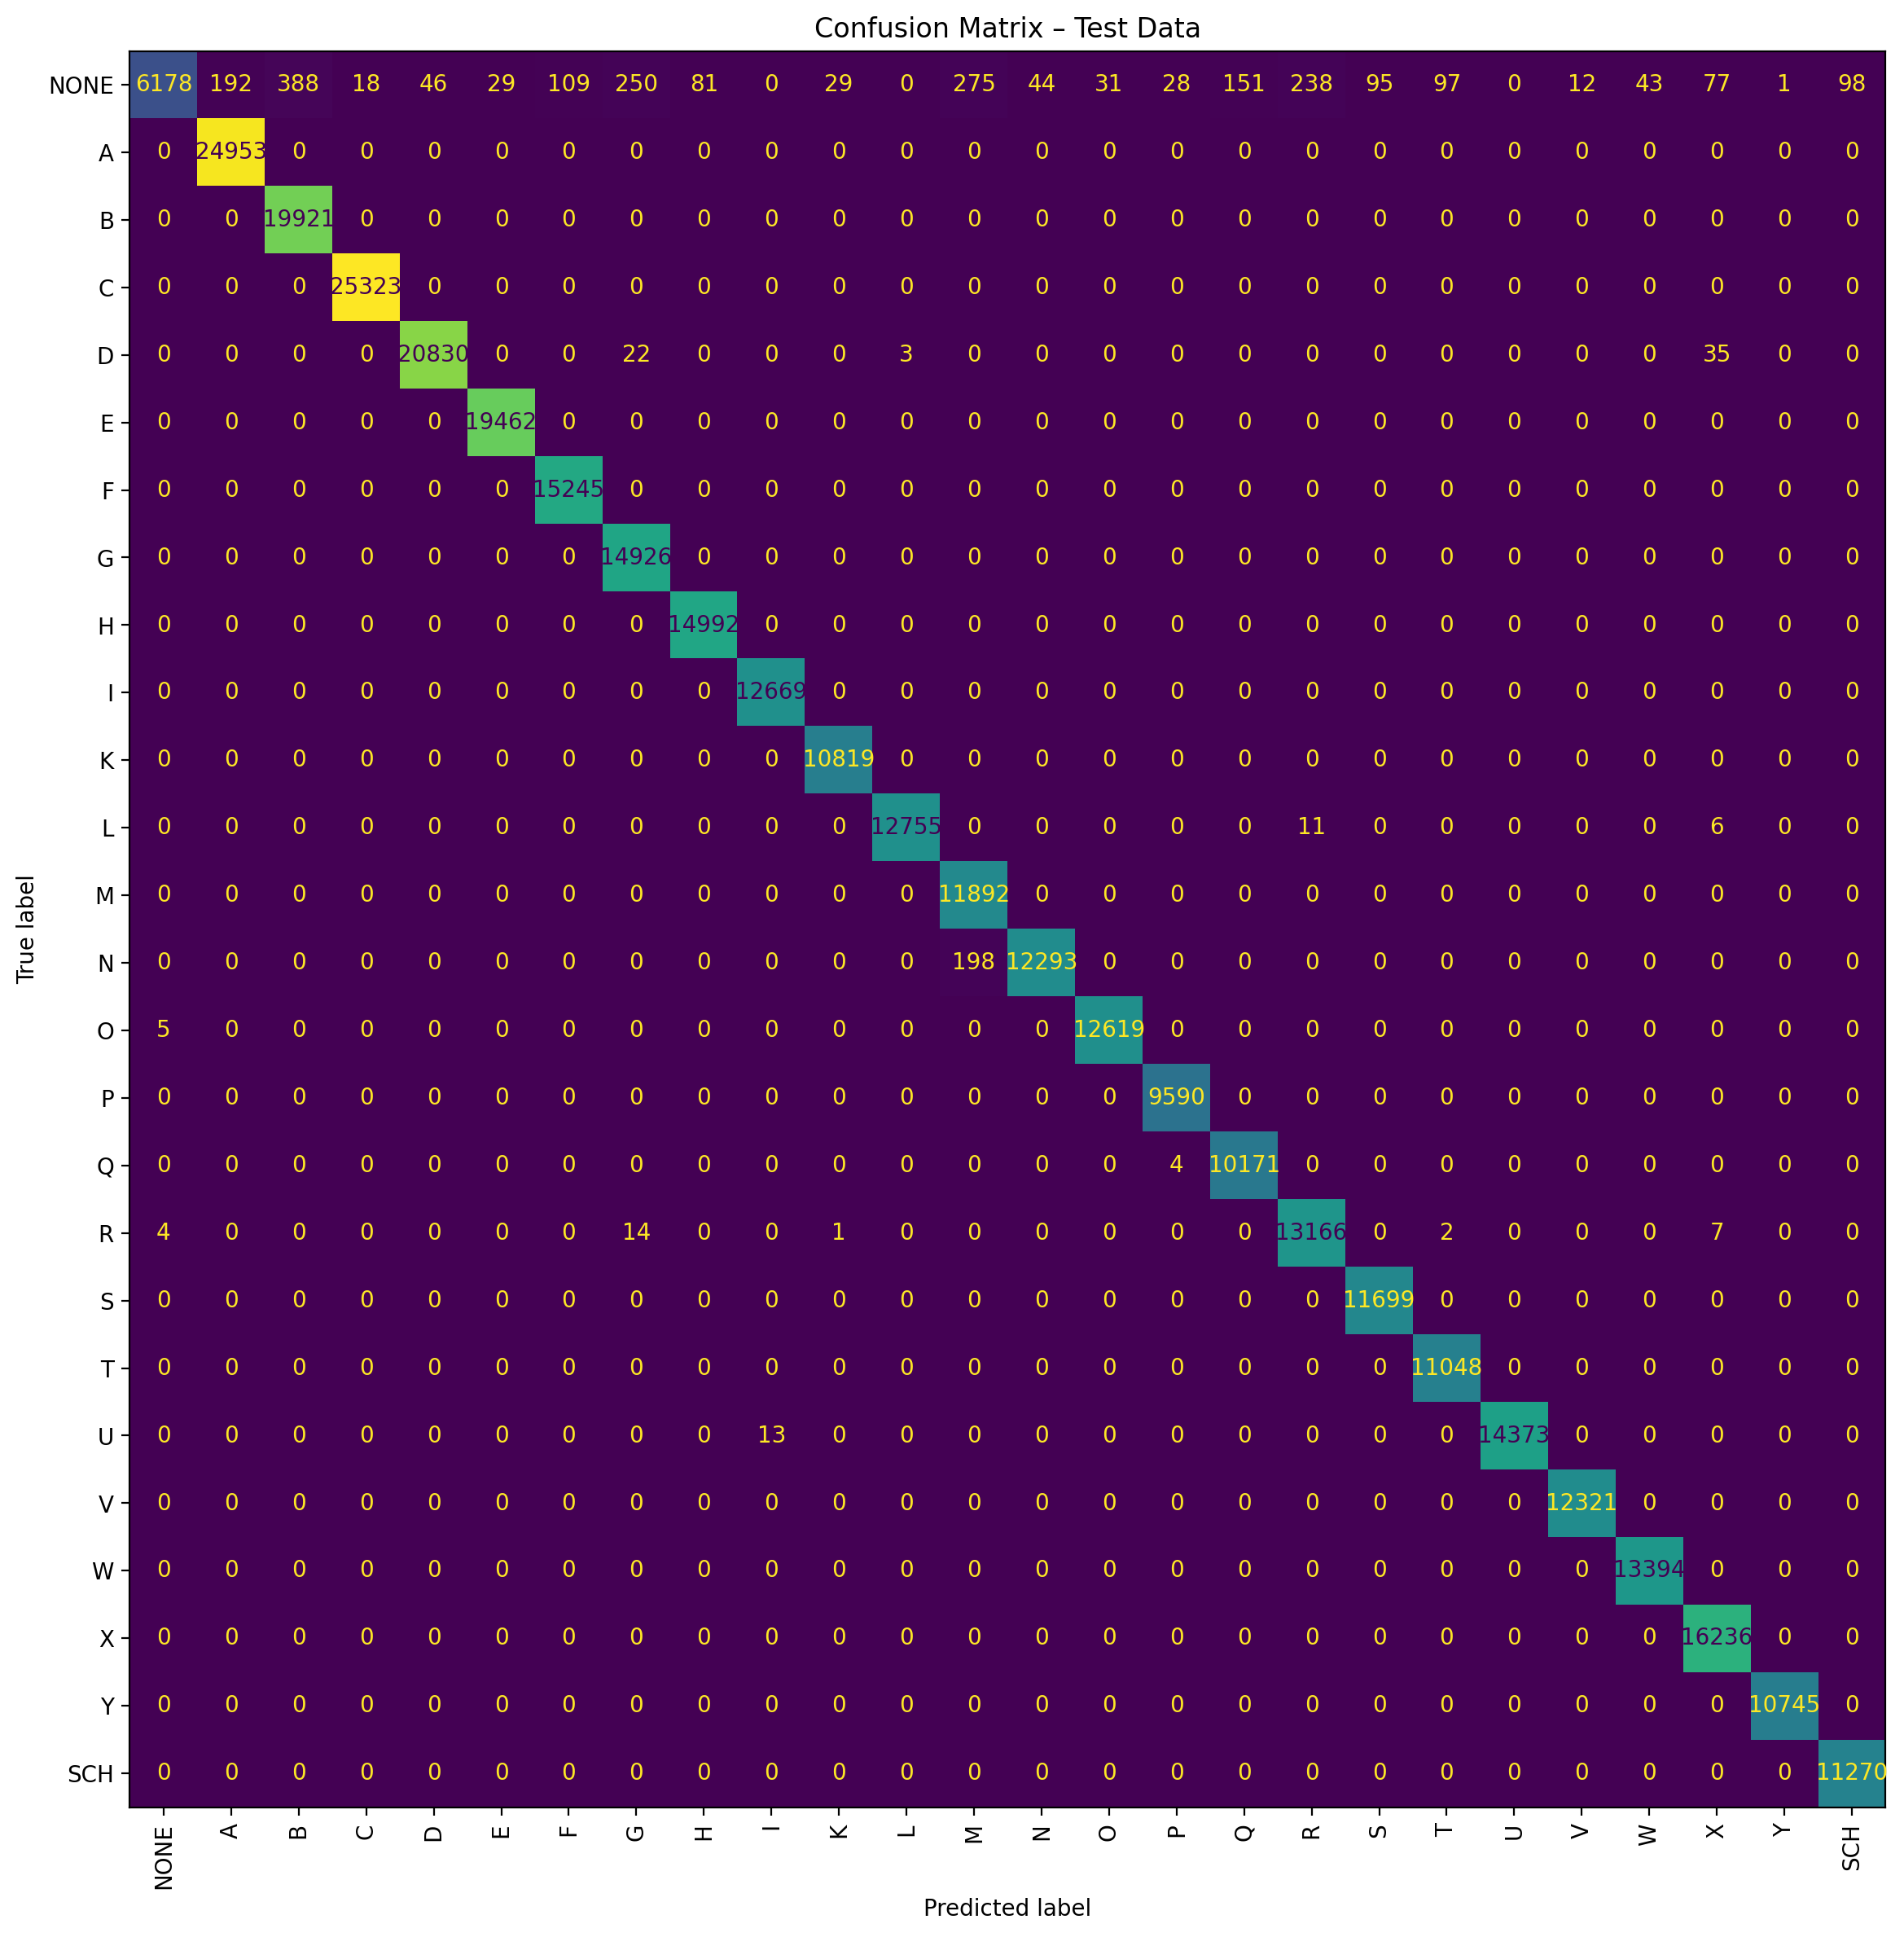
\includegraphics[width=0.4\textwidth]{material/figures/confusion_matrix.png}
    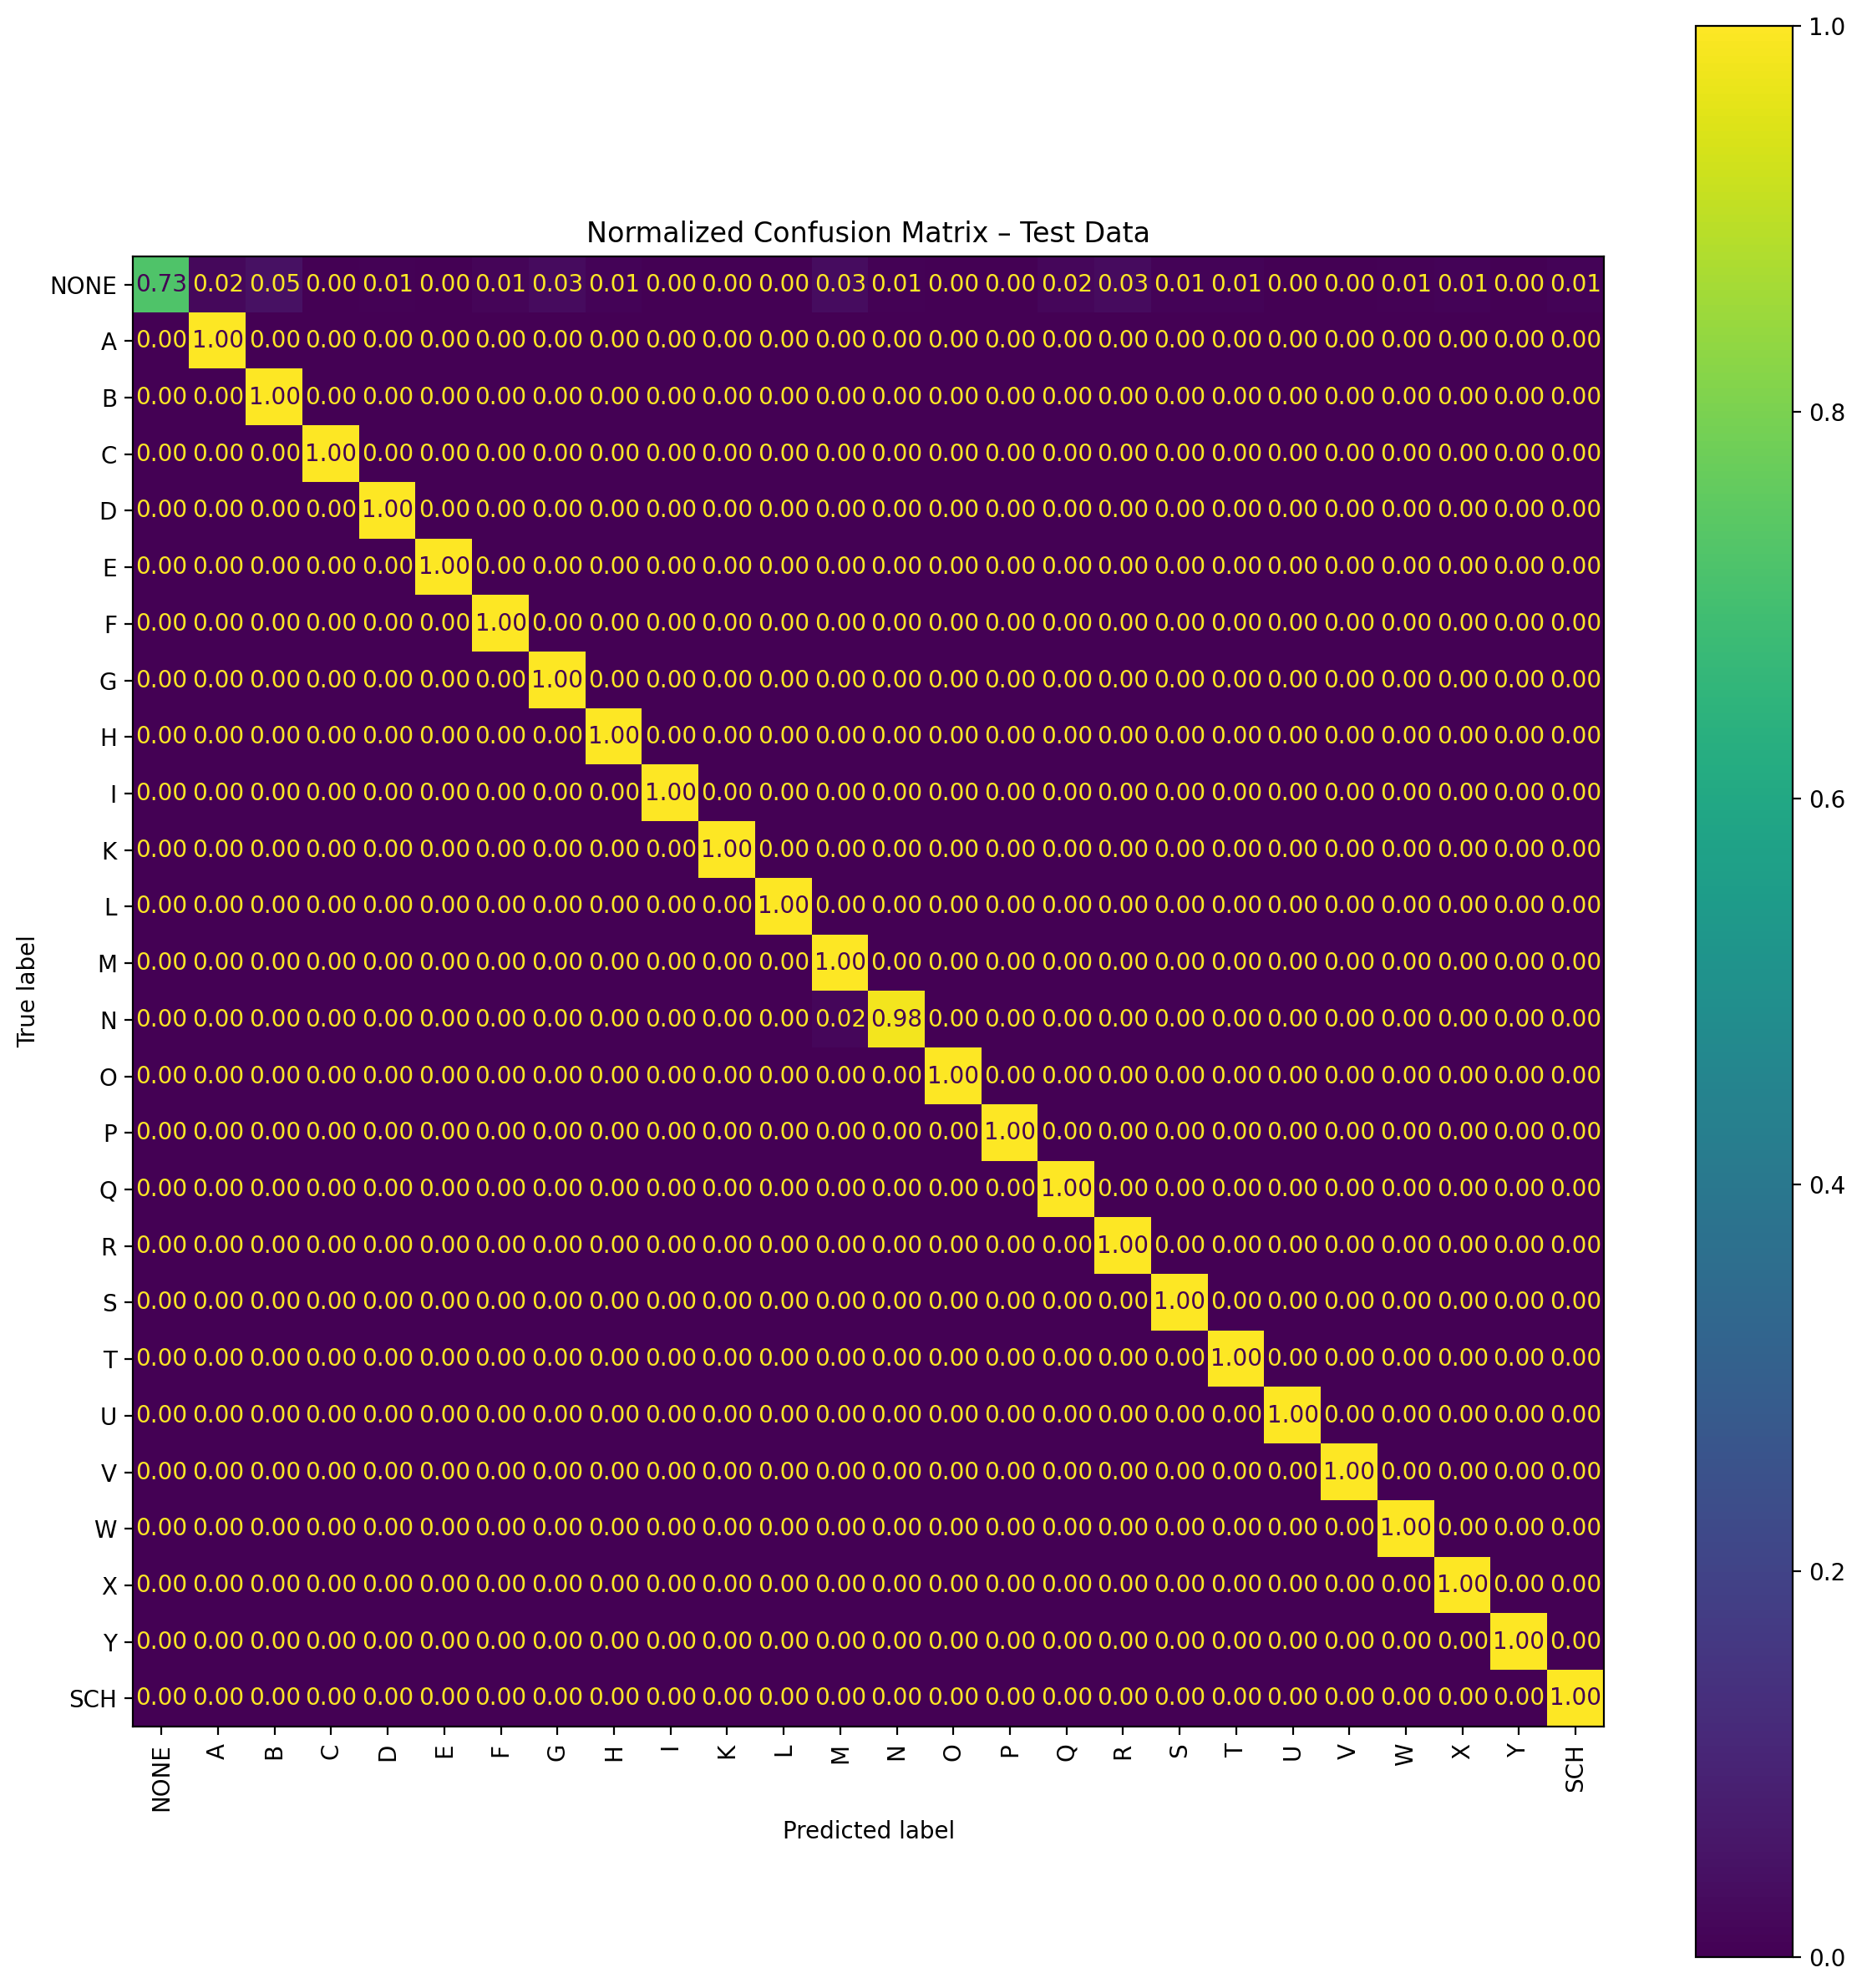
\includegraphics[width=0.4\textwidth]{material/figures/confusion_matrix_normalized.png}
    \caption{Roh und Zeilennormierte Konfusionsmatrix}
    \label{fig:confusion-matrix}
\end{figure}

Die Konfusionsmatrizen basierent auf 371.547 Testdaten mit einer 99,28\% Accuracy.
Die Matrix zeigt verschiedene Probleme des Modells auf.
\texttt{NONE} (Klasse 0) ist mit 72,6\% die mit Abstand schwächste Klasse. Sie wird häufig mit B (\texttt{388x} | 5\%), G, M, R (jeweils ca. \texttt{275x} | 3\%), A (2\%) und D,F,H,N,S,T, W, X, SCH (jeweils ca. \texttt{50} | 1\%) verwechselt. Es werden leere/ungesehene Hände oft als Buchstaben klassifiziert.
 Die Buchstaben N und M sind sich handgeometrisch sehr ähnlich (beide Faust mit ausgestreckten Fingern) und dadurch verwechselt (N $\rightarrow$ M \texttt{198x}). Eine weitere ausführlichere Aufschlüsselungen im Anhang \ref{tab:confusion-matrix}

 Das Modell ist bis auf NONE zuverlässig (99-100\% auf 24 von 26 Klassen). Die \texttt{NONE}-Erkennung ist mit \~73\% der größte Schwachpunkt.
 
\subsection{Praktischer Versuch zur Erkennungsgenauigkeit}\label{sec:praktischerversuch}

\subsubsection{Versuchsaufbau und Testbedingungen}\label{sec:versuchsaufbau}

Das System wird während der Versuche in einer festen Position aufgestellt. Die Handzeichen werden einzeln innerhalb des Erfassungsbereichs der Kamera dargestellt. Um die Versuche Vergleichbar zu gestalten, werden der Abstand zur Kamera, die Beleuchtung, der Hintergrund und die Anzahl der Wiederholungen dokumentiert. Die Bedingungen blieben während der gesamten Versuchsreihe unverändert.

\begin{longtable}{|p{0.4\textwidth}|p{0.45\textwidth}|}
    \caption{Grundlegende Bedingungen der Systemevaluation}
    \label{tab:versuchsbedingungen} \\
    \hline
    \texttt{Parameter} & \texttt{Festlegung} \\
    \hline
    \endfirsthead
    \hline
    \multicolumn{2}{r}{\texttt{Fortsetzung auf nächster Seite}} \\
    \endfoot
    \hline
    \endlastfoot
    Abstand zur Kamera & 50 -- 60 cm \\
    \hline
    Hintergrund & leer, weiße Wand \\
    \hline
    Beleuchtung & Lichtquelle von oben, außerhalb des Bildes \\
    \hline
    Unterstützte Zeichenklassen & SCH, NONE, A-Y ohne J \\
    \hline
    Versuchspersonen & acht \\
    \hline
    Wiederholungen je Zeichen &  fünf \\
    \hline
\end{longtable}

\subsubsection{Versuchsdurchführung}\label{sec:versuchsdurchfuhrung}

Der Feldversuch wurde mit acht anonymisierten Versuchspersonen unter den festgelegten Bedingungen durchgeführt. Die Versuchspersonen positionierten ihre rechte Hand im Zentrum des Kamerabildes. Der Körper befand sich seitlich außerhalb des für die Erkennung relevanten Bildbereichs, sodass sich hinter der dargestellten Hand ausschließlich die weiße Wand befand.

Vor der Aufzeichnung erhielt jede Versuchsperson für jedes Handzeichen einen nicht gewerteten Testversuch. Dieser diente dazu, die jeweilige Handform zunächst auszuprobieren und die Positionierung vor der Kamera zu überprüfen. Anschließend wurde das Handzeichen geformt und für drei Sekunden möglichst ruhig gehalten. Nach Ablauf dieser Zeit wurde das vom System ausgegebene Klassifikationsergebnis im Versuchsprotokoll dokumentiert. Nach jedem Einzelversuch wurde die Hand vollständig aus dem Erfassungsbereich der Kamera entfernt. Dadurch wurde das vorhandene Landmark-Tracking zurückgesetzt, sodass der folgende Versuch erneut mit der Handdetektion begann und unabhängig vom vorherigen Durchlauf ausgewertet werden konnte.

Dieser Ablauf wurde für jedes Zeichen fünfmal wiederholt. Danach wurde mit der nächsten Zeichenklasse fortgefahren. Bei 25 untersuchten Zeichenklassen, acht Versuchspersonen und fünf Wiederholungen je Zeichen ergaben sich insgesamt 1000 gewertete Einzelversuche. Die protokollierten Soll- und Ist-Klassen bilden die Grundlage für die Berechnung der Erkennungsgenauigkeit und die Erstellung der Konfusionsmatrix des Feldversuchs.

\subsubsection{Versuchsergebnisse}\label{sec:versuchsergebnisse}

Von den insgesamt 1000 durchgeführten Einzelversuchen wurden 912 Handzeichen korrekt klassifiziert. Dies entspricht einer Gesamterkennungsgenauigkeit von 91,2\,\%. In 57 Fällen wurde eine falsche Zeichenklasse ausgegeben. Bei weiteren 31 Versuchen lag nach der festgelegten Wartezeit kein gültiges Klassifikationsergebnis vor. Diese Fälle wurden ebenfalls als nicht erfolgreiche Erkennungen gewertet.

\begin{longtable}{|p{0.55\textwidth}|p{0.25\textwidth}|}
    \caption{Gesamtergebnis der praktischen Evaluation}
    \label{tab:gesamtergebnis-praktische-evaluation} \\
    \hline
    \textbf{Metrik} & \textbf{Ergebnis} \\
    \hline
    \endfirsthead
    \hline
    \textbf{Metrik} & \textbf{Ergebnis} \\
    \hline
    \endhead
    \hline
    \endlastfoot
    Durchgeführte Einzelversuche & 1000 \\
    \hline
    Korrekte Klassifikationen & 912 \\
    \hline
    Falsche Klassifikationen & 57 \\
    \hline
    Versuche ohne gültiges Ergebnis (NONE) & 31 \\
    \hline
    Gesamterkennungsgenauigkeit & 91,2\,\% \\
    \hline
\end{longtable}

Die Erkennungsleistung unterschied sich zwischen den einzelnen Zeichenklassen. Die Zeichen C, E, R, Y und SCH wurden in allen 40 Versuchen korrekt erkannt. Ebenfalls hohe Ergebnisse von mindestens 95\,\% erreichten B, F, I, L, T, U und X. Die geringste Erkennungsgenauigkeit wurde für das Zeichen M mit 52,5\,\% festgestellt. Von den 40 dargestellten M-Zeichen wurden 19 als N klassifiziert. Damit bildet die Verwechslung von M und N die deutlich häufigste Fehlklassifikation des Versuchs.

Weitere auffällige Verwechslungen traten zwischen V und R sowie zwischen A und S auf. Das Zeichen V wurde in sechs Fällen als R klassifiziert. Bei A erfolgte viermal eine Zuordnung zu S. Für das Zeichen H wurde eine Genauigkeit von 75\,\% erreicht; dabei wurde es unter anderem viermal als G klassifiziert. Das Zeichen D erreichte mit 80\,\% genau den zuvor festgelegten Mindestwert der Abnahmekriterien. Auch zwischen den Versuchspersonen zeigten sich Unterschiede. Die personenbezogene Erkennungsgenauigkeit lag zwischen 83,2\,\% und 95,2\,\%. Damit erreichten alle acht Versuchspersonen eine Erkennungsgenauigkeit oberhalb des festgelegten Mindestwerts von 80\,\%. Die Unterschiede weisen jedoch darauf hin, dass die individuelle Ausführung der Handzeichen einen Einfluss auf das Erkennungsergebnis besitzt.

Ergänzend zu den protokollierten Klassifikationsergebnissen wurden während der Versuchsdurchführung qualitative Beobachtungen zum Verhalten der Verarbeitungskette festgehalten. Wiederholt zeigte sich, dass sich die dargestellte Region of Interest während des Landmark-Trackings verkleinerte oder vollständig zusammenbrach. In diesen Fällen konnte die Hand teilweise nicht weiterverfolgt und folglich kein gültiges Klassifikationsergebnis ausgegeben werden. Dieses Verhalten wurde insbesondere bei einzelnen Versuchspersonen sowie bei einer vergleichsweise kleinen dargestellten Hand beobachtet. Damit können die Instabilitäten des Landmark-Trackings einen Teil der 31 Versuche ohne gültiges Ergebnis erklären.

Darüber hinaus wurden vereinzelt sprunghafte Landmark-Positionen und ein Flackern einzelner Fingerlandmarks festgestellt. Solche Schwankungen verändern die an das Klassifikationsmodell übergebenen Merkmale und können deshalb zu wechselnden Klassifikationsergebnissen führen. Bei den Zeichen A und S traten ebenfalls wiederholt Verwechslungen auf. Die Versuchsbeobachtungen deuten darauf hin, dass die Orientierung der Hand gegenüber der Kamera einen Einfluss auf die Unterscheidung dieser ähnlichen Handformen haben könnte. Vergleichbare Effekte wurden auch beim Zeichen I vermutet.

Die Beobachtungen zeigen insgesamt, dass die Erkennungsleistung nicht ausschließlich vom Klassifikationsmodell abhängt. Auch die Stabilität der Landmark-Erkennung und der Tracking-Region sowie die Größe, Orientierung und Ausführung der Handzeichen beeinflussen das Ergebnis der integrierten Verarbeitungskette. Diese Einflüsse werden bei der Interpretation der Ergebnisse in Kapitel~\ref{ch:diskussion} erneut aufgegriffen.

\subsection{Vergleich der Konfusionsmatritzen}\label{matrixvergleich}

Die normalisierten Konfusionsmatrizen zeigen deutliche Unterschiede zwischen der isolierten Auswertung des Klassifikationsmodells und der praktischen Evaluation des Gesamtsystems. Auf dem Testdatensatz wurden nahezu alle untersuchten Zeichenklassen vollständig korrekt erkannt. Lediglich das Zeichen N wurde in 2\,\% der Fälle als M klassifiziert. Im praktischen Versuch wurde dagegen eine Gesamterkennungsgenauigkeit von 91,2\,\% erreicht und es traten mehrere zusätzliche klassenbezogene Verwechslungen auf.

\begin{figure}[H]
    \centering
    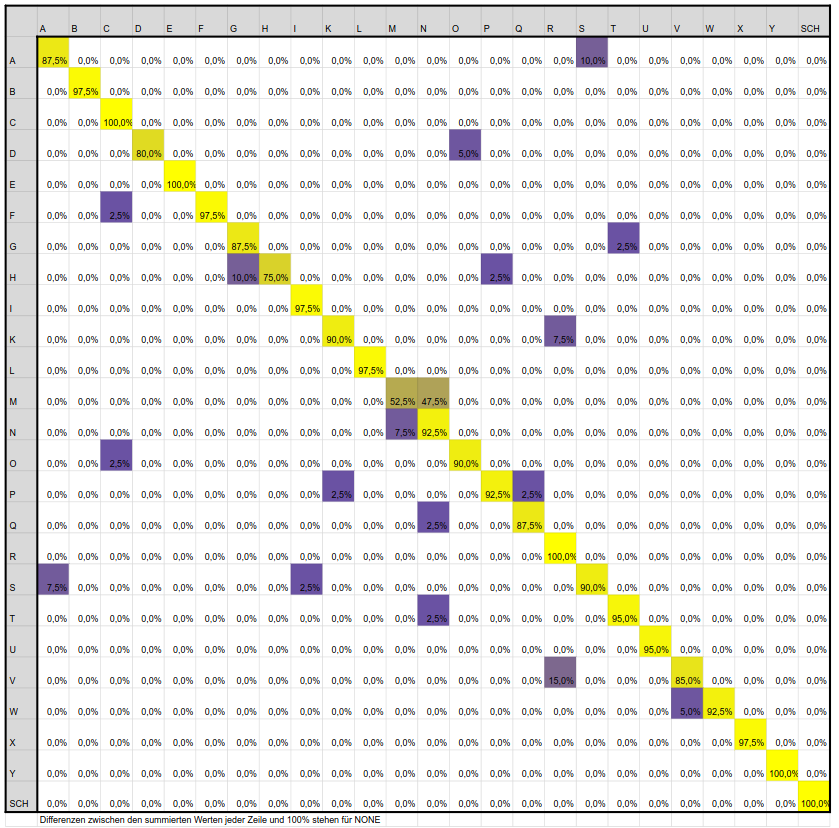
\includegraphics[width=0.5\linewidth]{material/figures/prak_confusion.png}
    \caption{Normierte Versuchs-Konfusionsmatrix}
    \label{fig:konfversuch}
\end{figure}

Die stärkste Abweichung zeigt sich beim Zeichen M. Während sämtliche M-Beispiele des Testdatensatzes korrekt klassifiziert wurden, erreichte die Klasse im praktischen Versuch lediglich eine Genauigkeit von 52,5\,\%. Die übrigen 47,5\,\% wurden vollständig der Klasse N zugeordnet. Umgekehrt wurde N im praktischen Versuch zu 7,5\,\% als M erkannt. Die bereits im Testdatensatz erkennbare Ähnlichkeit zwischen beiden Klassen verstärkte sich somit unter den praktischen Aufnahmebedingungen deutlich. Weitere im Testdatensatz nicht vorhandene Verwechslungen traten zwischen A und S sowie zwischen V und R auf. A wurde im praktischen Versuch zu 10\,\% als S erkannt, während S zu 7,5\,\% als A klassifiziert wurde. Das Zeichen V wurde zu 15\,\% der Klasse R zugeordnet. Demgegenüber wurden die Klassen C, E, R, Y und SCH in beiden Auswertungen vollständig korrekt erkannt. Auch B, F, I, L und X zeigten im praktischen Versuch mit jeweils 97,5\,\% nur eine geringe Abweichung gegenüber dem Testdatensatz.

Zusammenfassend zeigt der Vergleich, dass die hohe Erkennungsleistung auf dem Testdatensatz im praktischen Gesamtsystem nicht für alle Zeichenklassen gleichermaßen 
erreicht wurde. Die Abweichungen konzentrieren sich auf einzelne Klassenpaare, während ein
Großteil der Zeichen weiterhin zuverlässig erkannt wurde. Die möglichen Ursachen für die 
Unterschiede zwischen der isolierten Modellauswertung und der praktischen Evaluation werden in Abschnitt~\ref{sec:interpretation} diskutiert.

\section{Einfluss von Beleuchtung und Hintergrund}\label{sec:beleuchtung}
Ergänzend zur praktischen Evaluation wurde untersucht, welchen Einfluss eine sichtbare Lichtquelle und der Hintergrund im Kamerabild auf die initiale Handdetektion und das anschließende Landmark-Tracking besitzt. Eine Bewertung der Zeichenklassifikation erfolgte in diesem Versuch nicht. 

\subsection{Einfluss von Beleuchtung}

Für diesen Versuch wurden die zuvor verwendeten Versuchsbedingungen beibehalten. Zusätzlich wurde aber eine weitere Lichtquelle in verschiedenen Bereichen des Bildes hinzugefügt. Nach jedem Durchlauf wurde die Hand aus dem Kamerabild entfernt.

Ohne sichtbare Lichtquelle im Kamerabild wurde die Hand wie vorgesehen detektiert und das Landmark-Tracking anschließend stabil ausgeführt. Befand sich die Lichtquelle innerhalb des Kamerabildes, verschlechterte sich insbesondere die initiale Detektion. Der stärkste Einfluss wurde bei einer mittigen Positionierung der Lichtquelle beobachtet. Die Hand wurde in dieser Situation teilweise verzögert oder nicht erkannt, sodass die nachfolgende Verarbeitungskette nicht gestartet werden konnte. Lichtquellen im linken oder rechten Bildbereich beeinträchtigten die Detektion ebenfalls, der beobachtete Einfluss war jedoch geringer als bei der mittigen Positionierung.

\subsection{Einfluss des Hintergrunds}


\section{Inferenzlatenz und Ende-zu-Ende-Latenz}\label{sec:inferenzlatenz}
Ausgabe der Logs
\section{Bildrate und Datendurchsatz}\label{sec:bildrate}
Framerate berechnen. Datendurchsatz? Dazu fehlt mir noch die Idee

\section{Speicher- und Ressourcenverbrauch}\label{sec:speicherverbrauch}
Analog zum Memorypool. GGF Vergleich mit nicht quantisierten Modellen?
Aussplittung von Modellen (weights, ecblobs etc.)

\section{Abgleich mit den definierten Anforderungen}\label{sec:abgleich-anforderungen}
Tabelle für die Abnahmekritieren durchgehen, prüfen und sagen ob bestanden oder nicht.